\documentclass[a4paper,pdftex]{article}

\usepackage{array}
\usepackage{placeins}

\usepackage{hopsantut}
\usepackage{csquotes}

\hypersetup{pdfauthor={Robert Braun}, pdftitle={Hopsan Tutorial - Running an Optimization}, pdfsubject={Hopsan Tutorial}}

\begin{document}
\maketitle{Sensitivity Analysis}

\section*{Introduction}
In most simulations, it is impossible to know the exact value of all input parameters. 
As a consequence, there will be an uncertainty in the inputs, which will cause an uncertainty in the outputs. 
Sensitivity analysis is used to examine how the uncertainty in the output of a model is related to the uncertainty in the inputs.
In particular, it can be used for identifying how large impact on the result the uncertainty in each input parameter will have.
Sesitivity analysis can be performed in several ways.
In Hopsan it is performed by simulating the model for a large number of random input parameters, within specified limits. 
The results are then put together, and will be displayed as an area in the graph. 
This means that as long as the uncertainty of the inputs are within the specified limits, the output will always be somewhere within this area.

\section*{Step-By-Step Guide}
In this tutorial the sensitivity analysis tool will be demonstrated on a hydraulic linear servo with position feedback. We want to examine how the uncertainty in some different parameters will affect the step response. We will examine some parameters that are normally difficult to know, such as damping, leakage and valve overlaping.uliskt servo med positionsåterkoppling.

\begin{tutenumerate}

\tutitem{Open the model}
For this guide we will use the \textit{Position Servo} example model. It can be found from the welcome screen or from the help menu.

\tutitem{Open the sensitivity analysis dialog}
The sensitivity analysis dialog is opened from the icon in the toolbar:

\icon{0}{gfx/Hopsan-SensitivityAnalysis.png}{Open sensitivity analysis dialog (Ctrl-Shift-A)}

\tutitem{Choose settings}
In the bottom left of the dialog, it is possible to choose between normal and uniform distribution. It is also possible to set number of iterations. Choose uniform distribution and set number of iterations to 100.

\tutitem{Choose parameters}
Now we must choose which parameters we want to investigate. This is done in the list on the left side. We want to see how damping, leakage and valve overlaping affects the step response. Choose the following parameters:

{\renewcommand{\arraystretch}{1.2} 
\begin{tabularx}{\linewidth}{l X X}
\textbf{Parameter} & \textbf{Min} & \textbf{Max} \\
\specialrule{1.3pt}{0pt}{0pt}
4\_3\_Servo\_Valve, x\_at\#Value\hspace{50pt} & -1e-5 & 1e-5\\
4\_3\_Servo\_Valve, x\_bt\#Value & -1e-5 & 1e-5 \\
4\_3\_Servo\_Valve, x\_pa\#Value & -1e-5 & 1e-5 \\
4\_3\_Servo\_Valve, x\_pb\#Value & -1e-5 & 1e-5 \\
Cylinder\_C, B\_p\#Value & 0 & 1000 \\
Cylinder\_C, c\_leak\#Value & 0 & 1e-9 \\
Mass, B\#Value & 0 & 1000 \\
\end{tabularx}
}

\tutitem{Choose variables}
The selected parameters will affect the movement of the piston. To investigate this, choose the output value of the position sensor (\textit{Position\_Sensor, Out, Value}) in the right side list. If everything is correct, the dialog should look like the figure below:

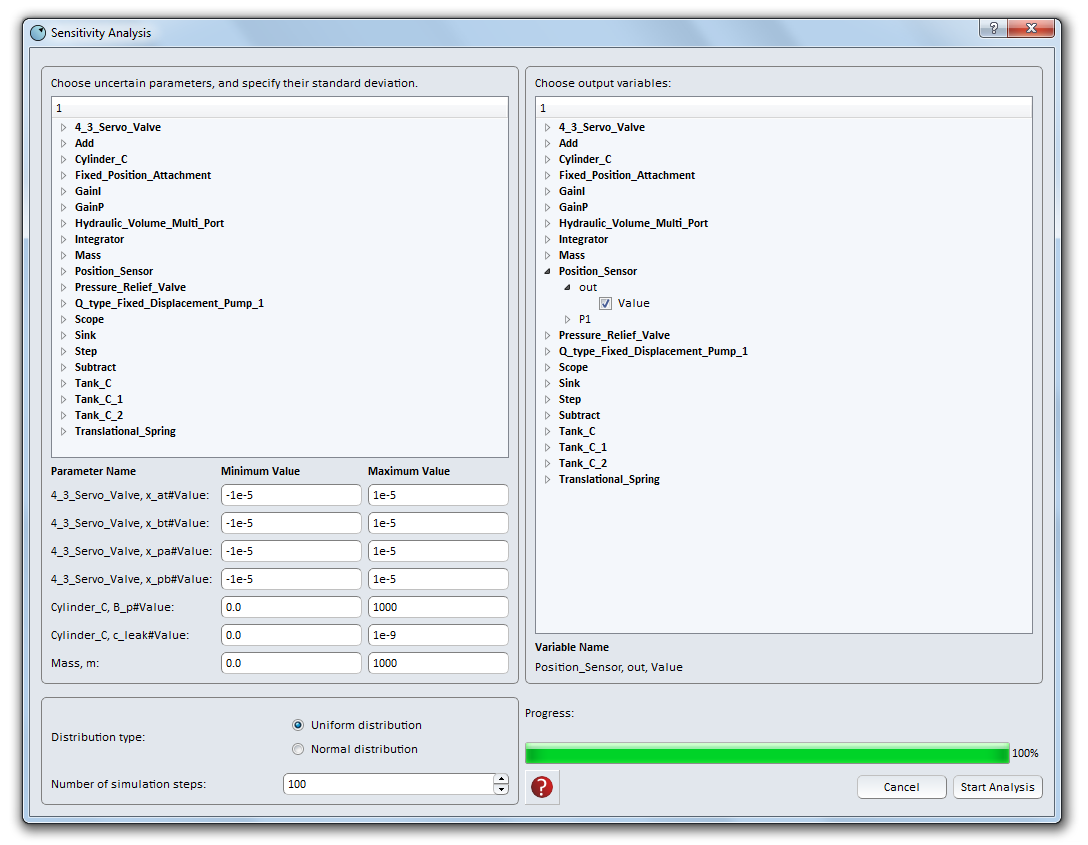
\includegraphics[width=\linewidth]{gfx/sensitivityanalysis/dialog.png}

\tutitem{Start the analysis}
Click on \textit{Start Analysis} to start the analysis. If your computer has a multi-core processor and if multi-threading is enabled in options dialog, parallel execution will be used to speed up the processes.

\tutitem{Examine the results}
The results show an area in the graph. This means that as long as all investigated parameters stay within their specified limits, the movement of the piston will be inside this area. It is thus for example possible to see the worst possible overshoot, rise time and settling time of the step response.

\end{tutenumerate}


\end{document}